\thispagestyle{fancy}
\chapter{Teori}
\label{chp:teori}

\section{Fysiologi}
\label{sec:fysiologi}
I projektet er der brugt den tidligere omtalte Myo, der er et wearable device fra Thalmic Labs. Myo'en bliver brugt til at optage data fra testpersoner. Dataene kan bruges til at træne machine learning modeller og anvende disse til udvikling af applikationer, der intuitivt kan reagere på elektromyografiske signaler fra armen.
I dette kapitel vil der blive givet et overblik over, hvordan aktiviteten i musklerne registreres. Der vil specifikt blive kigget på musklerne i underarmen, da det er signalerne herfra, der arbejdes med i projektet.


\myWrapFigure{myo}{Indersiden af Myo'en, hvor sensorerne har grænseflade til huden på underarmen. Myo'en placeres, hvor underarmen er tykkest for at få  det bedst mulige resultat. Der ses 3 pods, som hver er ens. Hver pod består af en EMG-sensor. På den midterste ses to store elektroder til at opfange signaler, mens den smalle i midten er til reference.}{fig:myo}{0.5}{r}

Når mennesket bevæger sig, sendes der signaler fra hjernen til rygmarven og herfra videre til de motoriske nerver (bevægenerverne), som til sidst overfører signalerne til musklerne. Musklerne i kroppen bliver aktiveret og trækker sig sammen, når de få signal til det. Det er en kombination af flere muskelgrupper i underarmen, der bevirker, at hånden og fingrene kan bevæges. Når muskelgrupperne på underarmens bøjeside aktiveres, fremkalder det først og fremmest bøje-bevægelser i håndled og fingre. Modsat når muskelgrupperne på underarmens strækkeside aktiveres, så fremkalder det overvejende udstrækning af håndled og fingre. Musklerne er opbygget af mange små muskelfibre. Når disse modtager elektriske signaler fra nerverne, trækker de sig sammen og dermed også hele musklen. Det er netop de elektriske signaler, der forårsager disse sammentrækninger i musklerne, der i projektet bliver opsamlet data på. De elektriske signaler kan opsamles med en Myo. Myo'ens sensorer består hver af en plus-elektrode og en minus- elektrode og en reference-elektrode. Reference-elektroden adskiller plus- og minus- elektroden. Se figur \ref{fig:myo}

De to elektroder måler de elektriske signaler fra muskelfibrene under muskelaktiviteten\citep{RefWorks:13}. Første og anden elektrode på samme sensor sidder placeret uden på huden og kan derfor både sidde på samme muskel, men også hvor muskler overlapper hinanden. Når der opsamles data med Myo'en, bliver EMG-signalerne bearbejdet af Myo'en, der giver en integer som output pr. sample for hver EMG-sensor. Output har ingen enhed, men er en approksimation af aktivitet, der er over sensoren ved sampling. På figur \ref{fig:anatomy} kan det ses, hvordan musklerne sidder i armen. Det er altså muligt at have en EMG-sensor til at sidde delvist på den muskel, der er markeret med gult og delvist på den muskel, der er markeret med grønt.

\myFigure{anatomy}{Bøjeside af venstre underarm med markering af muskler. Det ses, hvordan forskellige muskler hæfter forskelligt i håndleddet og dermed har hver sin funktion i hånden. Den grønne muskel kan være den, der ved sammentrækning bøjer tommelfingeren, mens den blå ved sammentrækning bøjer håndleddet.}{fig:anatomy}{1}

Når Myo'en tages på, kan den sidde på forskellige måder på armen, dog skal den sidde, hvor armen er tykkest. Dette betyder, at en sensor kan sidde på den med rødt markerede muskel én gang, og næste gang den tages på, kan den måske sidde på den med gult markerede muskel. Da musklerne er forbundet til hver sin funktionalitet i hånden, vil der komme to forskellige udfald i de opsamlede data. Der skal derfor tages højde for Myo'ens placering på armen, når der opsamles data.\\
Dette bliver nærmere beskrevet i sektion \ref{sec:optagelsedata}.

\section{Machine Learning}
\label{sec:machineLearning}
I følgende sektion vil den grundlæggende teori for brugen af machine learning blive belyst. Machine learning er læren om at få computere til at selv at "tænke"' uden rent faktisk at programmere dem.

Formålet med machine learning er, at lade et program lære af opsamlet data, i stedet for at programmere det. Der er tre typer af machine learning\citep{PatternBishop}:
\begin{description}
	\item[Supervised learning] er hvor træningsdata inputtet sammen med det ønskede output gives til computeren. Her bliver den altså lært hvilket output et givet input passer til.
	\item[Unsupervised learning] er derimod hvor der gives træningsdata, men ikke et tilhørende matchene output. Her er det altså op til computeren at finde et mønster, og dermed at kunne genkende lignede mønstre ud fra træningsdataene.
	\item[Reinforcement learning] er hvor computeren befinder sig i et dynamisk miljø og der skal findes løsninger for at komme nærmest målet. Reinforcement learning er bl.a. brugt i selvkørende biler.
\end{description}

I dette projekt er der arbejdet med supervised learning. Der bliver opsamlet data fra Myo'en og fortalt hvad inputtet er, og dermed også hvad den skal give af output. Inputtet er et specifikt datasæt der bliver opsamlet. Den specifikke data skal bruges til at genkende et mønster på noget nyt data. Dette kaldes \textit{induktion}, det specifikke skal bruges til at genkende det generelle. Omvendt er \textit{deduction} at gå den anden vej, fra det generelle til det specifikke.

\subsection{Proces}
Når et problem løses med machine learning, gøres det gennem en række steps. Der skal først loades data der er blevet opsamlet. Dernæst bliver den opsamlede data pre-processeret. Under præ-processeringen findes dataenes features. En feature er et kendetegn data har. Når dataene er klar, bliver de lært hvilket ouput de er mappet til. Dette er supervised learning. Det giver en model der kan anvendes til mønstergenkendelse. På figur \ref{fig:mlprocess} ses processen fra loading af data til trænet model \citep{MLMadeEasy}.

\myFigure{mlprocess}{I pre-processeringen af dataene bruges feature extraction for at klargøre dataene. Features er elementer der kendetegner dataene. Mere om dette i sektion \ref{sec:featurex}. Nu er dataene klar til at blive trænet. Med supervised learning, bliver det mappet til et output. Dette giver en Machine learning model. Pre-processering og træning af model, er en iterativ proces, hvor der prøves forskellige machine learning algoritmer}{fig:mlprocess}{1}

Nu er modellen lavet er klar til at lave mønstergenkendelse. Som det ses på figur \ref{fig:mlprocess2}, er det første der sker, det samme som bliver gjort under træning af en ny model. Derefter køres det igennem modellen som giver resultater på dataene.

\myFigure{mlprocess2}{Der bliver opsamlet data, som bliver pre-processeret. Disse to steps er det samme som gennemgået inden træning af en model. Når data er præ-processeret bliver de nu kørt igennem modellen, der løber alle dataene igennem og laver genkendelse på dem.}{fig:mlprocess2}{1}

\subsection{Problematik}
Når der trænes machine learning modeller, er det ikke altid at de laver genkendelse helt korrekt, som planlagt. To problemer man kan støde på ved en model er \textit{overfitting} og \textit{underfitting}. Overfitting opstår hvis der er for mange features. Modellen prøver derfor "for meget"' på at ramme hver enkel sample. Underfitting sker hvis der er for få features, der kendetegner dataene. Er det tilfældet, vil modellen ikke kunne lave successfuld genkendelse, da den ikke har haft nok informationer at gå ud fra.
%Kurve med validationsfejl kontra fejl/ fejl på træningssættet. 

\subsubsection{Over- og Underfitting}
Hvis der er lavet en kompleks model der er meget fleksibel og specifik, kan den være overfittet. På figur \ref{fig:over}\citep{fitting} ses et eksempel af en model med overfitting. Umiddelbart ser den ud til at være god, da den går gennem næsten alle samples. Problemet er, at den afviger meget fra den funktion, der er datasamples fra. Derfor kan den lave outputs der ligger langt fra målet. På figur \ref{fig:under}, ses det modsatte eksempel. På denne model ses underfitting. Modellen er en lige linje langs de samplede data, men den mister en masse samples, da den ligger for langt fra hver datasample.

\mySubFigure{overfitting}{underfitting}{Overfitting og underfitting. Det ses hvordan begge modeller har deres svagheder. Modellen på \ref{fig:over} har stor risiko for at "genkende"' for mange data som sit mål. Dog finder den alle de rigtige. På modellen på \ref{fig:under} derimod, finder den ikke de samples den bør, og genkender dermed ikke de mål den bør. }{}{}{fig:fitting}{fig:over}{fig:under}

%\begin{figure}[ht]
%	\centering
%	\subbottom[{}\label{fig:over}]%
%	{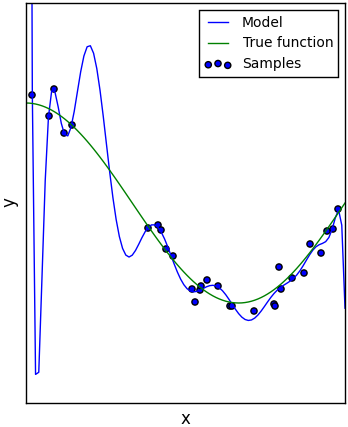
\includegraphics[width=0.4\textwidth]{overfitting}}
%	\subbottom[{}\label{fig:under}]%
%	{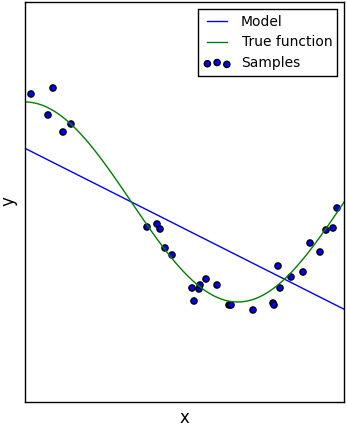
\includegraphics[width=0.4\textwidth]{underfitting}}
%	\caption{Overfitting vs. underfitting. Det ses hvordan begge modeller har deres svagheder. Modellen på \ref{fig:over} har stor risiko for at "genkende" for mange data som sit mål. Dog finder den alle de rigtige. På modellen på \ref{fig:under} derimod, finder den ikke de samples den bør, og genkender dermed ikke de mål den bør.}
%	\label{fig:fitting}
%\end{figure}



%Varians - sensitivitet over for individuelle data punktet i træningssæt, fejl i træningssættet
%Bias - 

\subsection{Løsninger}
For at undgå overfitting skal man sørge for ikke at have for mange features i træningsdataene. De kan evt. fjernes manuelt, så man udvælger hvilke der skal bruges og hvilke der ikke skal.
Når der trænes i MATLAB er der valideringsmetoder, der sørger for at reducere overfitting.
En metode er \textit{Cross-Validation}, her deles datasættet op i mindre stykker, hvor én del bruges til test, og resten til træning, se figur \ref{fig:crossval}. Man vælger selv hvor mange foldninger der skal bruges. Denne type validering er bedst til mindre datasæt på under 6000 observationer.

\myFigure{crossval}{I dette tilfælde der der valgt 3 foldninger. Datasættet deles derfor også op i 3 lige store dele, hvor én af dem bruges til test mens de to andre bruge til træning. Dette gøre 3 gange, hver gang hvor et nyt subset bruges til test.}{fig:crossval}{0.9}

En anden måde at mindske overfitting på er ved at bruge \textit{Holdout-validation}. Ved denne validering vælges der en procentdel af datasættet som bruges til test, resten laves der en model på. Dermed bliver modellen valideret. Holdout-validation er god til store mængder data på over 6000 observationer.

Med disse valideringsmetoder, bliver det muligt at se på sin model, om den er brugbar.










